\begin{figure}[h]
\begin{center}
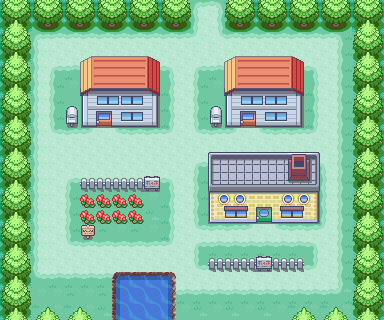
\includegraphics[width=2in]{PokemonPalletTown.png}
\end{center}
\caption{Pallet Town map from Pok\'{e}mon FireRed \cite{firered}}
\label{fig:pokemon}
\end{figure}

\begin{table}
\label{table:symbols}
\caption{Symbol names and the hand drawn forms}
\begin{center}
\begin{tabular}{llll}
Water & 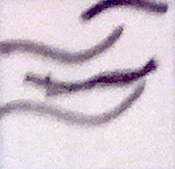
\includegraphics[width=.5in]{water.png} &
Grass & 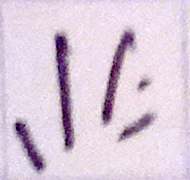
\includegraphics[width=.5in]{grass.png} \\
Rock & 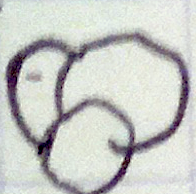
\includegraphics[width=.5in]{rocks.png} &
Tree & 
\includegraphics[width=.5in]{tree.png} \\
Dirt & 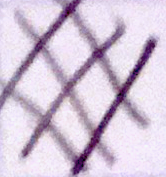
\includegraphics[width=.5in]{dirt.png} &
Sand & 
\includegraphics[width=.5in]{sand.png} \\
\end{tabular}
\end{center}
\end{table}


The maps used for classification in this project are hand drawn on standard 4 to 1" grid paper using a custom set of symbols defined for this purpose. These maps vary in cell dimensions and distribution of symbols but are all derived from the popular video game Pok\'{e}mon. This was done to ensure that proximity information and terrain types were standard throughout. In total, 10 different maps were used with a total of 13488 cells each containing one symbol. An example map from the game is shown in Figure \ref{fig:pokemon}.  The custom symbol set consists of 7 symbols created to represent the terrain types needed to build the maps in Pok\'{e}mon. These symbols are: water, dirt, grass, building, rock, mountain and sand and can be seen in \ref{table:symbols} . Each symbol was made to be visually distinct from each of the other symbols to help with classification. By choosing a specific source such as this we ensure that our dataset is sampled from a well defined distribution.


